%%%%%%%%%%%%%%%%%%%%%%%%%%%%%%%%%%%%%%%%%%%%%%%%%%%%%%%%%%%%%%%
% Part of EBESS and MESS Presentation: Learn to LaTeX 2019
% Prepared by JT
% March 2019
%%%%%%%%%%%%%%%%%%%%%%%%%%%%%%%%%%%%%%%%%%%%%%%%%%%%%%%%%%%%%%%
\documentclass[]{article}
\usepackage{graphicx} % this one is important

\title{Graphics and floats}
\author{Joshua Tambunan}
\date{\today}

\begin{document}
\maketitle

% example of including images and using optional arguments
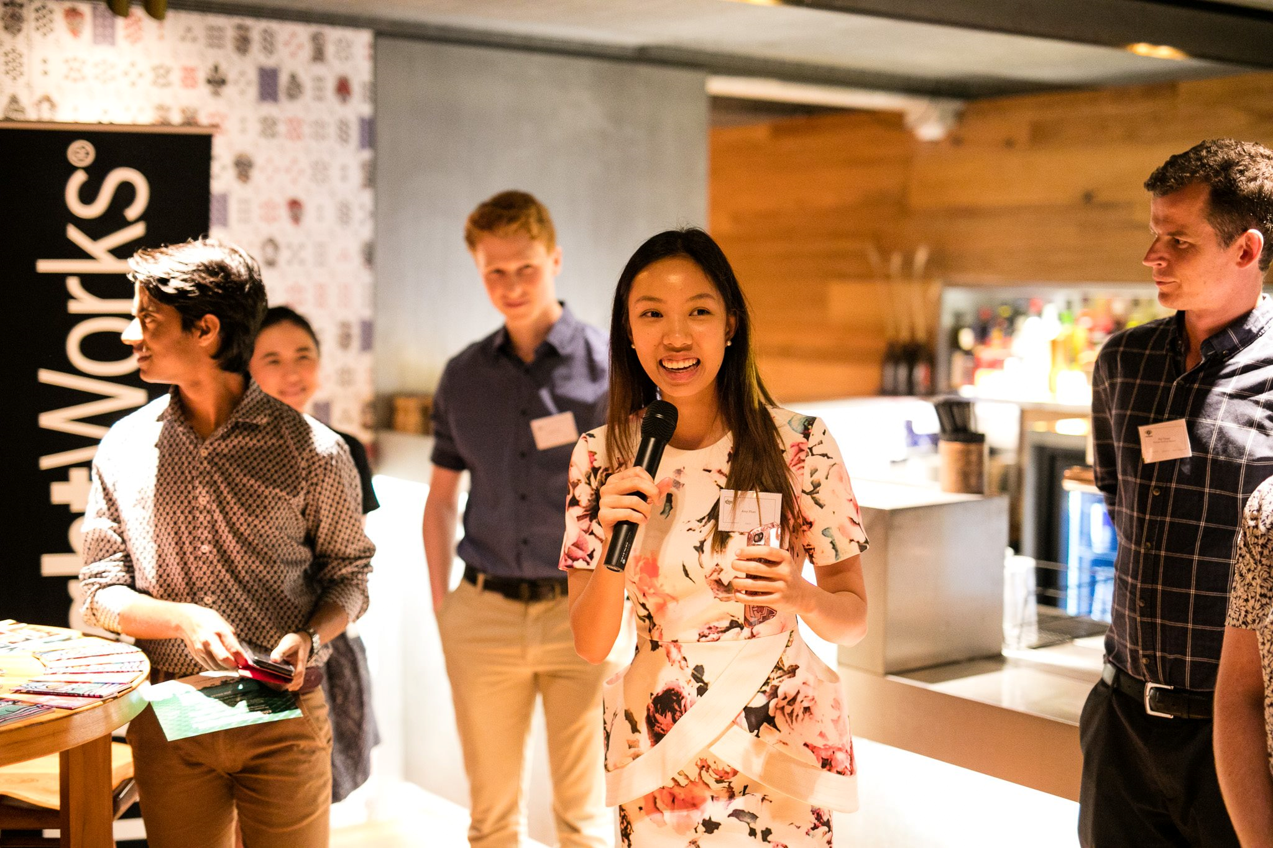
\includegraphics[
    width=0.5\textwidth]{../img/employ.png}
    
% float: let's add caption
Figure \ref{fig:amy} shows the ex-secretary of EBESS in her habitat: a networking event.
\begin{figure}
    \centering
    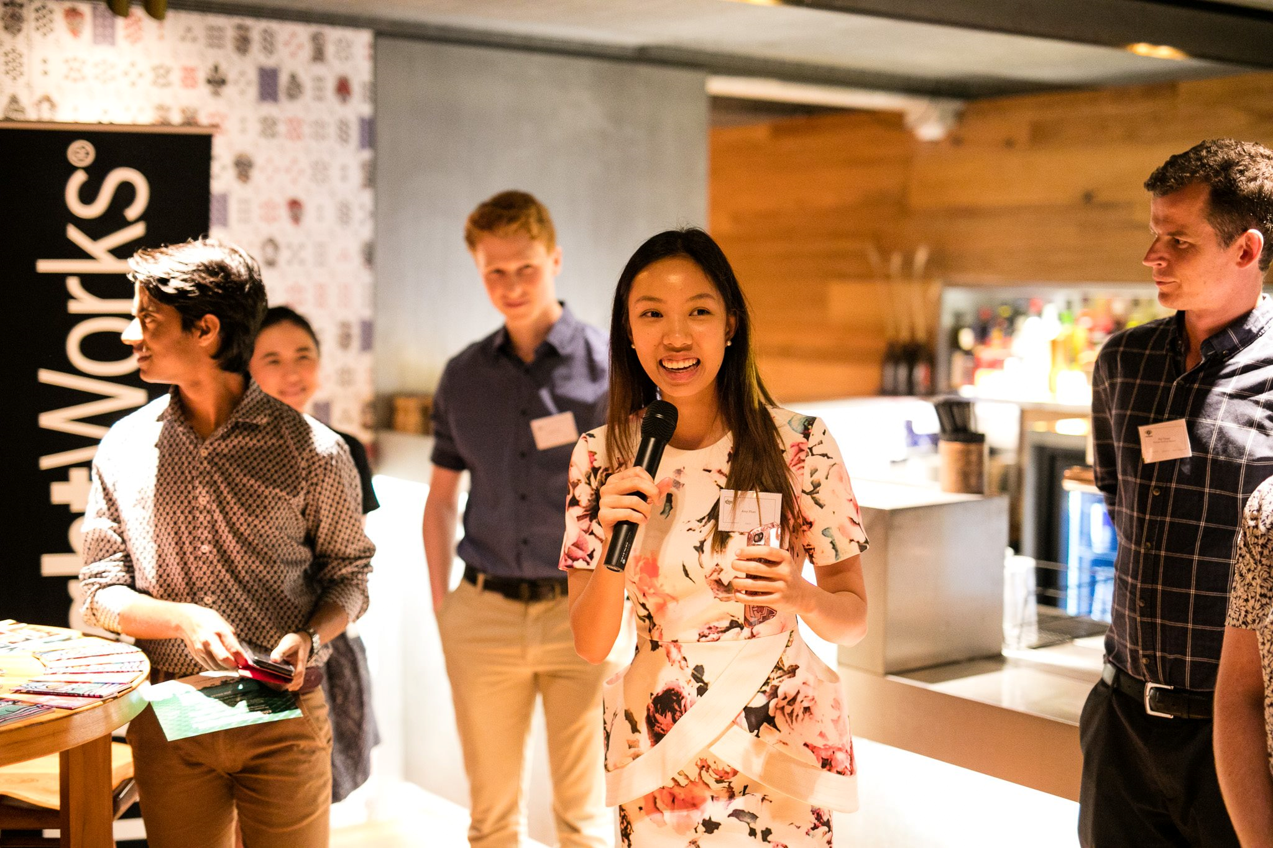
\includegraphics[%
        width=0.5\textwidth]{../img/employ.png}
    \caption{\label{fig:amy}The lovely Amy Phan}
    \label{fig:my_label}
\end{figure}

% Why did LaTeX do that to me?

\end{document}